\chapter{Timbre Similarity} \label{musly}

\textit{MFCCs explained in chapter 1, here: how many melbands, visualize GMM}\\
Proposed methods according to \cite[pp.51ff]{knees1}\\
Mel Frequency Cepstral Coefficients have already been introduced in chapter \ref{mfccsim}. This chapter focuses on the different similarity metrics.\\
To reduce the dimensionality of the data even further, a statistical summarization of the MFCC feature can be calculated \cite[p. 58]{knees1}.
For each of the Mel- Bands (12 in this case) the mean and standard deviation over all frames is calculated, resulting in a vector of 12 mean values, a 12 by 12 co-variance matrix (actually $\frac{12*11}{2}$ values, because of the triangular shape - the upper triangle contains the co-variances and the main diagonal contains the variances) and 12 variances. These vectors are therefore not dependent on the length of the actual song. 
Using such a model, the distance between two songs can be calculated as in equation \ref{eq:distGmm}, where x and y are the n-dimensional feature vectors of two different musical pieces:
\begin{equation} \label{eq:distGmm}
%p (v \vert \lambda)=\sum_{i=1}^{M}w_iN(v \vert \mu_i,\sum_i) \label{prob}
d(x, y) = ||x - y||_p = \left(\sum_{i=1}^{n}{|x_i - y_i|^p}\right)^{\frac{1}{p}}
\end{equation}
also known as the $L_p$ distance. Most of the times, the Euclidean ($L_2$) or the Manhattan ($L_1$) distance would be used in real world scenarios.
This very basic approach has been refined and improved over the past years. 

\section{Single Gaussian Model}

This approach was first proposed by Mandel and Ellis \cite{mandelellis1} in 2005 and is briefly summarized in \cite[pp. 65f]{knees1}.\\
After computing the mean value of each MFCC ($\mu_P$ and $\mu_Q$) and the covariance matrix of the different MFCC vectors ($\Sigma_P$ and $\Sigma_Q$) of two musical pieces $P$ and $Q$, the Kullback-Leibler divergence (KL divergence) can be calculated as follows, with $Tr(\cdot)$ being the trace (i.e. the sum of the diagonal of a matrix), $d$ being the dimensionality (number of MFCCs) and $|\Sigma_P|$ being the determinant of $\Sigma_P$\\
\begin{equation} \label{eq:KL1}
KL_{(P||Q)} = \frac{1}{2}[log\frac{|\Sigma_P|}{|\Sigma_Q|} + Tr(\Sigma_P^{-1}\Sigma_Q) + (\mu_P - \mu_Q)^T \Sigma_P^{-1} (\mu_Q - \mu_P) - d]
\end{equation}
As a second step the result has to be symmetrized.
\begin{equation} \label{eq:KL2}
d_{KL}(P, Q) = \frac{1}{2} (KL_{(P||Q)} + KL_{(Q||P)}) 
\end{equation}
This approach is one of the two available similarity metrics of the musly \cite{musly1} toolkit introduced in section \ref{mirtoolkit}.
This can be simplified and written as a closed form:
\begin{equation} \label{eq:SKL}
d_{SKL}(P, Q) = \frac{1}{4} (tr(\Sigma_P\Sigma_Q^{-1}) + tr(\Sigma_Q\Sigma_P^{-1}) + tr((\Sigma_Q^{-1}\Sigma_P^{-1})(\mu_P - \mu2)^2) - 2d)
\end{equation}

\section{Other Similarity Metrics}
\textit{different similarity metrics, we use easiest one}\\
\ \\
\ \\
The second available metric in the musly toolkit by Schnitzer is using the Jenson-Shannon Divergence (in an slightly adapted way). "The Jensen-Shannon (JS) divergence is another symmetric divergence derived from the Kullback-Leibler divergence. To compute it, a mixture $X_m$ of the two distributions is defined" \cite[p. 43]{schnitzer1}. "To use the Jensen-Shannon divergence [...] to estimate similarities between Gaussians, an approximation of $X_m$ as a single multivariate Gaussian can be used [...] This approximation of $X_m$ is exactly the same as the left-type Kullback-Leibler centroid of the two Gaussian distributions [...]" \cite[p. 44]{schnitzer1} 
\begin{equation} \label{eq:jsl1}
\mu_m = \frac{1}{2} \mu_P + \frac{1}{2} \mu_Q
\end{equation}
\begin{equation} \label{eq:jsl2}
\Sigma_m = \frac{1}{2} (\Sigma_P + \mu_P\mu_P^T) + \frac{1}{2} (\Sigma_Q + \mu_Q\mu_Q^T) - \mu_m\mu_m^T
\end{equation}
\begin{equation} \label{eq:jsl3}
JS(P, Q) = \frac{1}{2} log|\Sigma_m| - \frac{1}{4} log |\Sigma_P| - \frac{1}{4} log |\Sigma_Q|
\end{equation}
After calculating a similarity matrix for all songs, it normalizes the similarities with mutual proximity (MP). \cite{musly2}  This method wants to reduce the effect of a phenomenon called hubness that appears as a general problem of machine learning in high-dimensional data spaces. "Hubs are data points which keep appearing unwontedly often as nearest neighbors of a large number of other data points." \cite[p. 66]{schnitzer1}.\\
Schedl and Knees state: "To apply MP to a distance matrix, it is assumed that the distances $D_{x,i = 1..N}$ from an object $x$ to all other objects in the data set follow a certain probability distribution; thus, any discance $D_{x,y}$ can be reinterpreted as the probability of $y$ being the nearest neighbor of $x$, given the distance $D_{x,y}$ and the probability distribution $P(x)$ [...] MP is then defined as the probability that $y$ is the nearest neighbor of $x$ given $P(x)$ and $x$ is the nearest neighbor of $y$ given $P(y)$" \cite[p. 80]{knees1}\\
Resulting in: 
\begin{equation} \label{eq:mp1}
P(X > D_{x,y}) = 1 - P(X \leq D_{x,y}) = 1 - \mathscr{F}(D_{x,y}) 
\end{equation}
\begin{equation} \label{eq:mp2}
MP(D_{x,y}) = P(X > D_{x,y} \cap Y > D_{x,y})
\end{equation}
according to \cite[p. 80]{knees1}
\ \\
Another, more compute heavy distance measurement would make use of Gaussian Mixture Models of MFCCs. As Knees and Schedl state "Other work on music audio feature modeling for similarity has shown that aggregating the MFCC vectors of each song via a single Gaussian may work almost as well as using a GMM [...] Doing so decreases computational complexity by several magnitudes, in comparison to GMM-based similarity computations." \cite[p. 65]{knees1} Therefore the usage of GMMs is not further considered in this thesis.
\ \\
The last method mentioned in this thesis for timbral similarity is to use block-level features as proposed by Seyerlehner \cite{seyerlehnerblock} and described in short by Knees and Schedl \cite[p. 67]{knees1}. 
Instead of using single frames and summarizing them into statistical or probabilistic models, block-level features use larger, e.g. multiple second long, audio frames and features like fluctuation patterns are computed for these frames. 

\section{Validation}

For this thesis the approach by Mandel and Ellis is used to compute the similarity matrix, because it is . There is always a trade-off of complexity and functionality. 
Using the musly toolkit, a first evaluation is presented in the next section. 
The feature extraction and distance calculation can also be done in python using the librosa library and a small reimplementation of the Mandel-Ellis approach was tested.\\
\textit{A possible measure for the efficiency of a timbre similarity algorithm is the ability to find songs of the same genre.}

\subsection{Construction Noise}
Comparing a construction noise sound sample with the private music collection containing mostly metal, rock, pop, classical and hip hop music, the following six best results could be achieved in descending order: 

\begin{itemize}
	\setlength\itemsep{0em}
	\item Ziegenm\"uhlen Session - Down On The Corner (Folk Musik)
	\item While She Sleeps - The Divide (Metalcore)
	\item Delain - Mother Machine (Live) (Symphonic Metal)
	\item Within Temptation - Sanctuary (Intro Live) (Symphonic Metal)
	\item Without A Martyr - Medusa's Gaze (Death Metal)
	\item 100 Meisterwerke der Klassik - Orpheus In The Underworld (Orph\'ee aux enfers) - Can-Can (Live At Grosser Saal, Musikverein) (Klassik)
\end{itemize}
Figure \ref{const1} and \ref{const2} show the distribution of the genres of 100 most similar songs compared to the construction noise sample.  

\begin{figure}[htbp]
	\centering
	\framebox{\parbox{1\textwidth}{ 
			\begin{subfigure}{0.49\textwidth}
				\centering      
				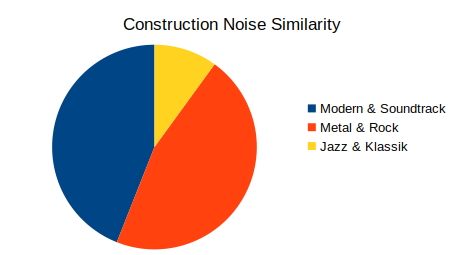
\includegraphics[scale=0.45]{Images/cnoise1.png}
				\caption{Similar genres to construction noise sample file}
				\label{const1}
			\end{subfigure}%
			\begin{subfigure}{0.49\textwidth}
				\centering 
				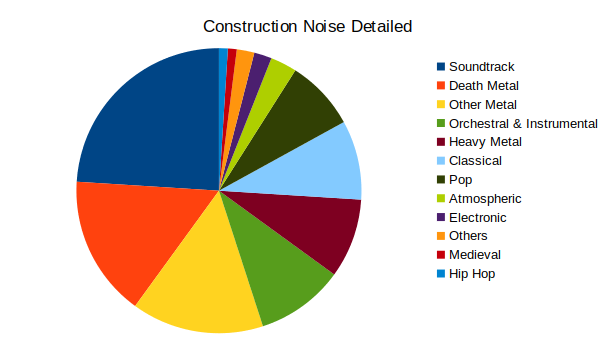
\includegraphics[scale=0.45]{Images/cnoise2.png}
				\caption{Similar genres to construction noise sample file in detail}
				\label{const2}
			\end{subfigure}
	}}
	\caption{Construction Noise}
	\label{fig:constn}
\end{figure}

Using the full dataset consisting of the private music collection, private field recordings, the full fma-dataset and the musicnet data, the following results could be achieved: 

\begin{itemize}
	\setlength\itemsep{0em}
	\item Born Pilot - Birds Fell (FMA, Electronic, Noise)
	\item mrandmrsBrian - sun is boring (FMA, Avant-Garde, field recordings)
	\item steps in snow (private field recording)
	\item Sawako - Paris Children (FMA, field recordings)
	\item Jeremy Gluck and Michael Dent - Olivier (FMA, Ambient Electronic)
	
\end{itemize}

\subsection{Different recordings and cover versions}
Another experiment was, to get the most similar songs to the famous 'Rondo alla Turca' by Mozart.
The recording used as a starting point is from the CD "100 Meisterwerke der Klassik" and has a length of 3:33 minutes.
This piece by Mozart appears overall four times in the dataset and is recorded by different pianists.
Every recording has a different length as listed in the following overview of the recordings by CD

\begin{itemize}
	\setlength\itemsep{0em}
	\item 100 Meisterwerke der Klassik (3:33)
	\item Piano Perlen (3:30)
	\item The Piano Collection - Disk 18 (3:28)
	\item Mozart Premium Edition - Disk 31 (4:29)
	
\end{itemize}
The top ten most similar songs to the 3 minutes and 33 seconds version are listed below:
\begin{itemize}
	\setlength\itemsep{0em}
	\item Mozart - Concert No. 10 for 2 Pianos and Orchestra in E Flat Major, KV 365 - 2. Andante
	\item Schubert - Sonata in B Flat, D. 960 - III. Scherzo (Allegro vivace con delicatezza)
	\item Albeniz - Iberia, Book I - Evocaci\'on
	\item Mozart Sonate Nr. 11 in A-Dur, K. 33 - Mozart - Alla Turca Allegretto (3:28)
	\item Beethoven - Bagatellen Op 119 -Allemande in D major
	\item Mozart - Rondo No. 1 in D Major, K. 485
	\item Mozart - Sonata For Piano No. 8 KV 310 A Minor - Allegro Maestoso
	\item Sonata For Piano No. 16 KV 545 C Major - Rondo: Allegretto
	\item Mozart Sonate Nr. 11 in A-Dur, K. 33 - III. Tuerkischer Marsch (3:30)
	\item Mozart - Piano Sonata No. 13 in B flat major, K. 333 (K. 315c): Allegretto grazioso
	
\end{itemize}

The interesting conclusion is that only 2 out of the 3 other versions were considered as most similar songs.
The slower recording wasn't even in the top 30 list of the most similar songs. 
The same was observable for other cover versions of songs in the dataset like Serj Tankians song "Lie Lie Lie" from the CD "Harakiri" and an orchestral recording of the same piece. 
This is probably due to the usage of GMMs of MFCCs representing and valuing the timbre of the music predominantly instead of the pitches and melody movements.





